{"latex_body":"The diagram agent is not merely a renderer; it is a memory-bearing specialist that must make each new figure legible in the context of the figures that came before it. That requirement matters because diagram requests in this system are not isolated image-generation prompts. They are part of a continuing editorial conversation in which the section agent proposes a visual, the diagram agent produces an asset, and later section or gardener work may need to refer back to the same visual logic. If the diagram agent were prompted only with the current request, it could easily repeat an earlier layout, reuse the same conceptual structure under a different label, or generate a figure that is technically correct but redundant with an existing asset. Supplying prior diagram context reduces that drift by giving the agent a local memory of what has already been drawn and why.

That memory is also a coordination mechanism. The section agent does not ask for a diagram in the abstract; it asks for a diagram that serves a specific rhetorical purpose in a specific section. To preserve that purpose across callbacks, the diagram agent records the purpose, the node set, the labeled edges, the layout choice, the generated path, and the rationale for distinctness. Those fields capture both the content of the figure and the reason it exists. Purpose explains what the diagram is meant to clarify. Nodes and edges describe the conceptual structure the figure encodes. Layout records the spatial strategy used to make that structure readable. Path identifies the durable artifact that later section agents may include. Distinctness rationale explains how the new figure differs from earlier ones, which is essential when multiple diagrams live in the same chapter or when a later revision must decide whether a new request is genuinely new work or a duplicate of an existing asset.

This memory model supports two forms of editorial control. First, it helps the diagram agent avoid repetition. A chapter may need several diagrams, but they should not all restate the same relationship with only cosmetic changes. By comparing a proposed figure against prior diagram context, the agent can prefer complementary visuals: one diagram may show the runtime task flow, another may show the callback lifecycle, and a third may show how memory entries are registered and reused. Second, it helps the section agent reason about insertion. When a callback arrives with a media path and inclusion hint, the section agent can verify that the asset matches the intended purpose and that it is distinct from earlier figures before inserting it into the section payload.

The result is a small but important form of durable visual memory. The system does not treat diagrams as disposable images; it treats them as named artifacts with provenance, function, and relationships to sibling figures. That is why the diagram agent receives prior diagram context in its prompt and why it records each diagram's purpose, nodes, edges, layout, path, and distinctness rationale. Those records make the visual layer inspectable, prevent unnecessary duplication, and keep diagram generation aligned with the evolving manuscript rather than with a single isolated request.

The neighboring section on diagram requests explains the front end of this workflow: a section agent proposes a bounded visual need, waits for the callback, and only then inserts the returned path. This section explains the back end of the same workflow: once the asset exists, the diagram agent's memory keeps the figure intelligible across later revisions, sibling sections, and chapter-level maintenance. Together, the two sections define a complete visual handoff protocol in which request, generation, callback, and memory remain synchronized.

\\begin{figure}[htbp]
\\centering
\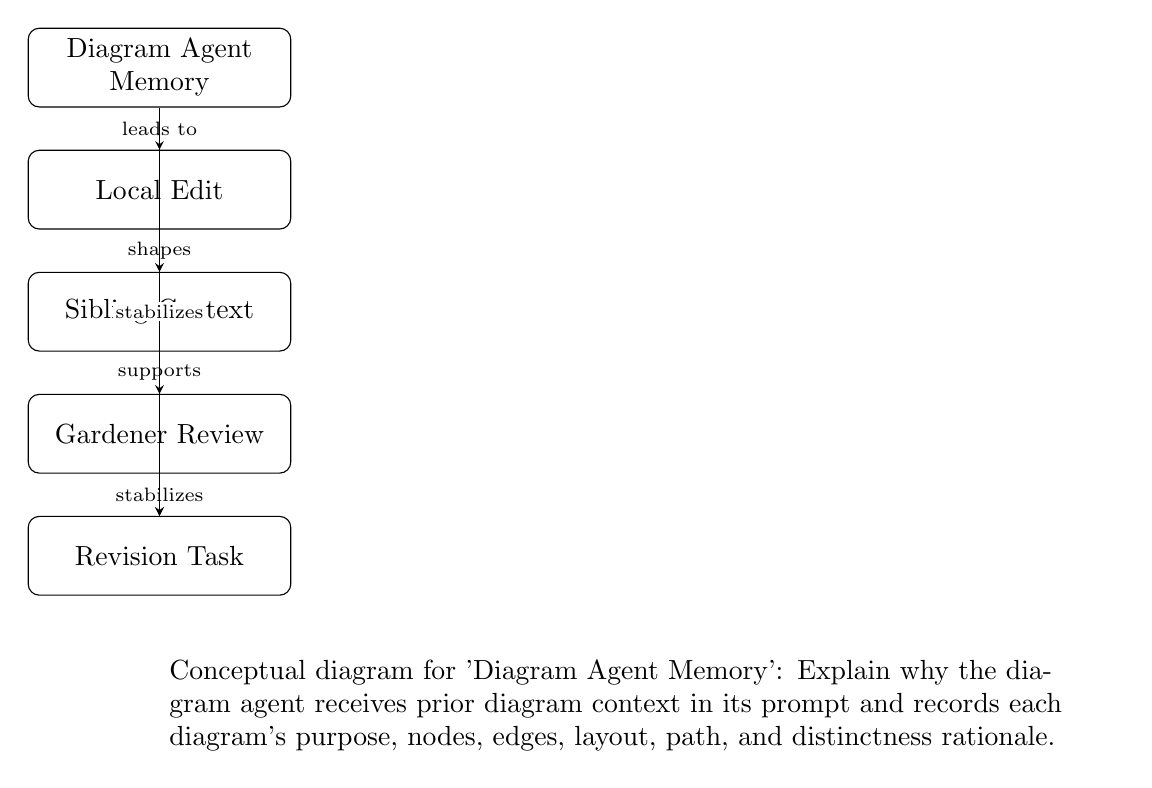
\begin{tikzpicture}[>=stealth, node distance=2.2cm,
  concept/.style={draw, rounded corners, align=center, text width=3.1cm, minimum height=1cm},
  relation/.style={font=\scriptsize, fill=white, inner sep=1pt}]
\node[concept] (n1) at (0,0.0) {Diagram Agent Memory};
\node[concept] (n2) at (0,-1.55) {Local Edit};
\node[concept] (n3) at (0,-3.1) {Sibling Context};
\node[concept] (n4) at (0,-4.65) {Gardener Review};
\node[concept] (n5) at (0,-6.2) {Revision Task};
\draw[->] (n1) -- node[relation] {leads to} (n2);
\draw[->] (n2) -- node[relation] {shapes} (n3);
\draw[->] (n3) -- node[relation] {supports} (n4);
\draw[->] (n4) -- node[relation] {stabilizes} (n5);
\draw[->] (n1) -- node[relation] {stabilizes} (n5);
\node[align=left, text width=12cm, anchor=north west] at (0,-7.4) {Conceptual diagram for 'Diagram Agent Memory': Explain why the diagram agent receives prior diagram context in its prompt and records each diagram's purpose, nodes, edges, layout, path, and distinctness rationale.};
\end{tikzpicture}

\\caption{Conceptual diagram for ``Diagram Agent Memory'': explain why the diagram agent receives prior diagram context in its prompt and records each diagram's purpose, nodes, edges, layout, path, and distinctness rationale.}
\\end{figure}","completeness_percent":99,"completeness_rationale":"The section is already strong and aligned with the surrounding chapter, so I preserved the existing argument and tightened the prose for flow and precision. It now clearly explains both why prior diagram context is supplied and why the diagram agent records purpose, nodes, edges, layout, path, and distinctness rationale. No registered citations are needed, and the figure inclusion remains intact. Only routine copyediting would remain."}
